%%%%%%%%%%%%%%%%%%%%%%%%%%%%%%%%%%%%%%%%%%%%%%%%%%%%%%%%%%%%%%%%%%%%%%%
%%%%%%%%%%%%%%%%%%%%%%%%%%%%%%%%%%%%%%%%%%%%%%%%%%%%%%%%%%%%%%%%%%%%%%%
%% start of file `simple-tikz-example.tex'.                          %%
%%                                                                   %%
%% Author: Daniel Sacré; date: 2022-01-20                            %%
%%                                                                   %%    
%% A very simple example for using node shapes and color mixing      %%
%% within tikz                                                       %%
%%                                                                   %%
%% LICENSE:                                                          %%
%% This work is released under Creative Commons Zero (CC0 1.0)       %%
%% into the public domain.                                           %%
%%%%%%%%%%%%%%%%%%%%%%%%%%%%%%%%%%%%%%%%%%%%%%%%%%%%%%%%%%%%%%%%%%%%%%%
%%%%%%%%%%%%%%%%%%%%%%%%%%%%%%%%%%%%%%%%%%%%%%%%%%%%%%%%%%%%%%%%%%%%%%%

\documentclass{standalone}

\usepackage{tikz}
\usetikzlibrary{shapes} % required for drawing outlines of nodes

% counter for addressing object position in grid
\newcounter{rows}
\newcounter{columns}
\setcounter{rows}{1}
\setcounter{columns}{1}

\begin{document}
	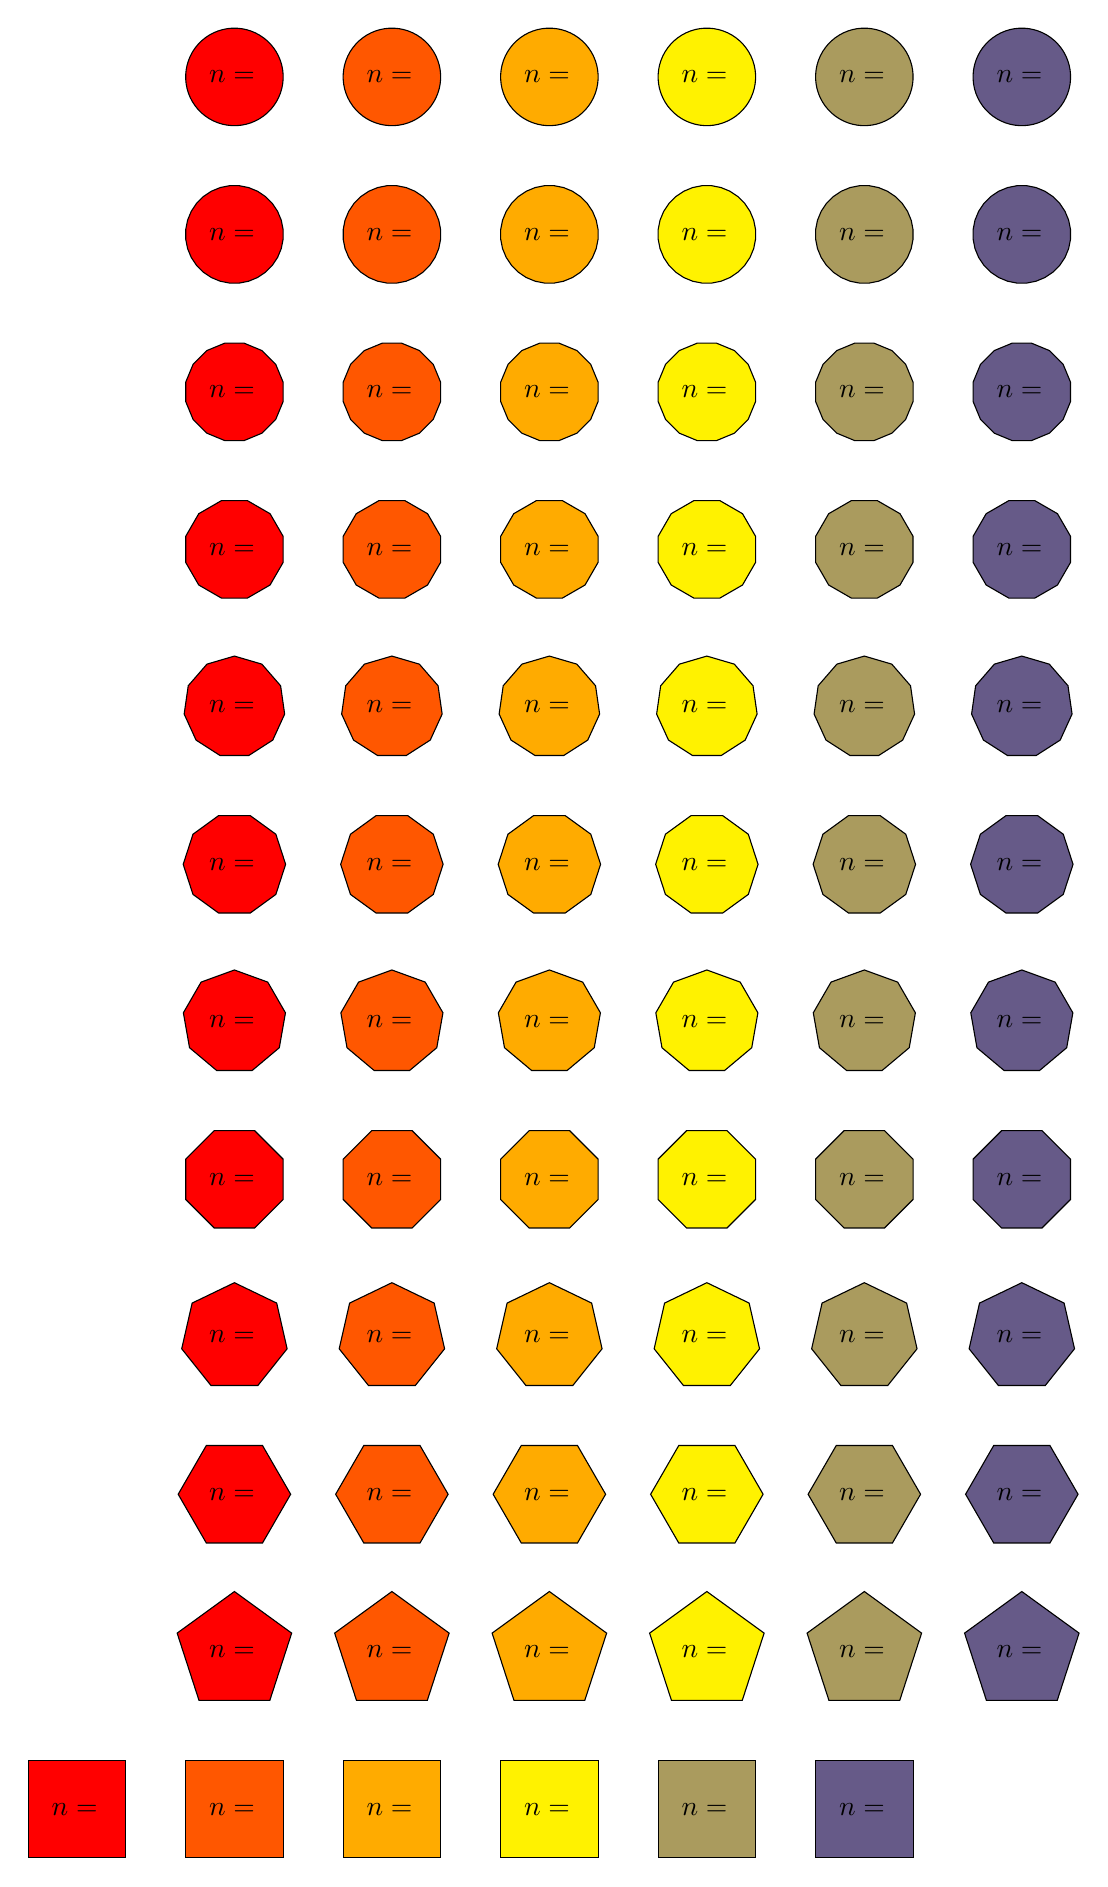
\begin{tikzpicture}
		\foreach \edgeCount in {4,5,...,12,16,32,64}{% iterate over all polygon edge counts
			\foreach \colorX/\colorY in {red/yellow, yellow/blue}{% iterate over all colors
				\foreach \mix in {100,66,33}{% iterate over all color mixing factors
					% draw node with \edgeCount polygon edges, fill it with color and
					% set node text to the number of polygon edges 
					\node[draw,fill=\colorX!\mix!\colorY,regular polygon,regular polygon sides=\edgeCount] at (2*\thecolumns,2*\therows) {$n=$\,\shape};
					\stepcounter{columns} % advance column position
				}
			}
			\setcounter{columns}{1} % reset column position
			\stepcounter{rows} % advance row position
		}
	\end{tikzpicture}
\end{document}
%%%%%%%%%%%%%%%%%%%%%%%%%%%%%%%%%%%%%%%%%%%%%%%%%%%%%%%%%%%%%%%%%%%%%%%
%%%%%%%%%%%%%%% end of file `simple-tikz-example.tex'. %%%%%%%%%%%%%%%%
%%%%%%%%%%%%%%%%%%%%%%%%%%%%%%%%%%%%%%%%%%%%%%%%%%%%%%%%%%%%%%%%%%%%%%%